\documentclass[english]{article}

\usepackage{ae,aecompl}
\usepackage[T1]{fontenc}
\usepackage[latin9]{inputenc}
\usepackage{textcomp}
\usepackage{graphicx}
\usepackage{eurosym}
\usepackage{hyperref}
\usepackage{float}

\makeatletter
\usepackage{babel}


\makeatother

\usepackage{babel}
\begin{document}
\begin{figure}
	\centering
	\includegraphics[scale=0.5]{logo.pdf} 
\end{figure}


\title{PowerEnJoy\\
 Requirement Analysis and Specification Document\\
}

\date{A.A 2016/2017}

\author{Erba Alessandro\\
 Leveni Filippo\\
 Lodi Luca}

\maketitle
\pagebreak{}

\tableofcontents{} \pagebreak{}

\section{Introduction}
	\subsection{Purpose }
	\subsection{Scope and Problem Description}
	\subsection{Goals}
	\subsection{Domain Assumptions }
	\subsection{Glossary}
		\subsubsection{User}
		An \textit{user} is a person subscribed to the PowerEnJoy service which can access to the car sharing through his smartphone.
	\subsubsection{Service}
		The \textit{service} is the group of actions that an \textit{user} can fulfill trough the mobile.
	\subsubsection {Safe Area}
		A \textit{safe area} is a  geographical place (defined by a set of GPS positions) on the map in which parking is allowed. \textit{safe areas} are saved into the system. An user can end a car sharing parking his car only in safe areas.
	\subsubsection{Power Grid}
		A \textit{power grid} is the object that charge the battery of an electric car. All \textit{power grid} are displayed in the	map. Each \textit{power grid} is in a \textit{safe area}, a user who plugs his car into a \textit{power grid} receives the 				discount provided by the Service.
	\subsubsection{Reservation}
		A \textit{reservation} is the possibility that a user has to "lock" a car at the latest for one hour.
	\subsection{Further Developments }
	We think that one of the most important things is to release a Service that can be extended and improved.
	For this purpose we will develop a system open to new extensions. \\
	E.g.:
	\begin{itemize}
		\item New discount policies can be introduced to the system, for example discounts for new users. 
		\item New system policies may be necessary.
		\item New kind of vehicles can be introduced, for example electric scooter and electric bikes.
		\item Allow new payment methods, for example Paypal\textregistered.
		\item Develop new services in order to increase the user experience, for example  allow communication among users in order to share a car ride and save money.
	\end{itemize}
	\subsection{Used Tools}

\section{Specific Requirements}
	\subsection{Functional Requirements}
	\subsection{Non Functional Requirements}

\section{Scenarios Identifying}
\section{UML Models And Use Cases}
	\subsection{Use Cases Diagram}
	\subsection{Actors Identifying}
	\subsection{Use Cases}

	\subsection{Class Diagram}
\section{External Interfaces}
\section{Alloy Model}
\section{Hours of Work}

\end{document}